\usetikzlibrary{calc}
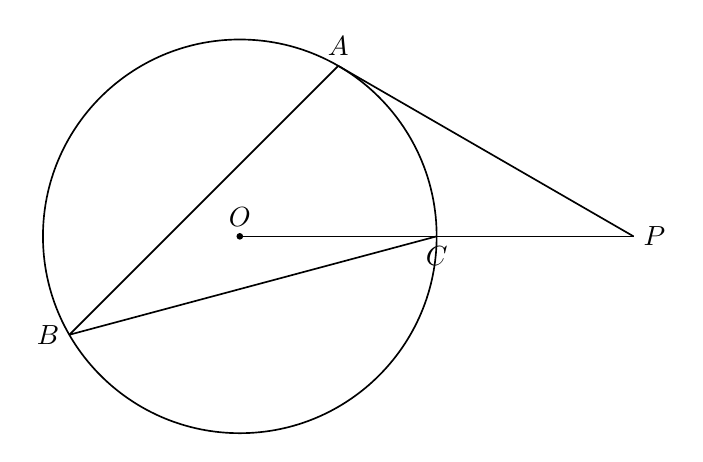
\begin{tikzpicture}[x=1cm,y=1cm,line width=.6pt,font=\normalsize]
\coordinate (O) at (0.0,0.0);
\coordinate (C) at (2.5,0.0);
\coordinate (A) at (1.25,2.16506);
\coordinate (B) at (-2.16506,-1.25);
\coordinate (P) at (5.0,0.0);
\draw (O) circle[radius=2.5cm];
\draw (A)--(B);
\draw (B)--(C);
\draw (O)--(P);
\draw (A)--(P);
\fill (O) circle[radius=1.2pt];
\node[above] at (O) {$O$};
\node[above] at (A) {$A$};
\node[left] at (B) {$B$};
\node[below] at (C) {$C$};
\node[right] at (P) {$P$};
\end{tikzpicture}
